% Options for packages loaded elsewhere
\PassOptionsToPackage{unicode}{hyperref}
\PassOptionsToPackage{hyphens}{url}
%
\documentclass[
]{article}
\usepackage{lmodern}
\usepackage{amssymb,amsmath}
\usepackage{ifxetex,ifluatex}
\ifnum 0\ifxetex 1\fi\ifluatex 1\fi=0 % if pdftex
  \usepackage[T1]{fontenc}
  \usepackage[utf8]{inputenc}
  \usepackage{textcomp} % provide euro and other symbols
\else % if luatex or xetex
  \usepackage{unicode-math}
  \defaultfontfeatures{Scale=MatchLowercase}
  \defaultfontfeatures[\rmfamily]{Ligatures=TeX,Scale=1}
\fi
% Use upquote if available, for straight quotes in verbatim environments
\IfFileExists{upquote.sty}{\usepackage{upquote}}{}
\IfFileExists{microtype.sty}{% use microtype if available
  \usepackage[]{microtype}
  \UseMicrotypeSet[protrusion]{basicmath} % disable protrusion for tt fonts
}{}
\makeatletter
\@ifundefined{KOMAClassName}{% if non-KOMA class
  \IfFileExists{parskip.sty}{%
    \usepackage{parskip}
  }{% else
    \setlength{\parindent}{0pt}
    \setlength{\parskip}{6pt plus 2pt minus 1pt}}
}{% if KOMA class
  \KOMAoptions{parskip=half}}
\makeatother
\usepackage{xcolor}
\IfFileExists{xurl.sty}{\usepackage{xurl}}{} % add URL line breaks if available
\IfFileExists{bookmark.sty}{\usepackage{bookmark}}{\usepackage{hyperref}}
\hypersetup{
  pdftitle={Borden},
  hidelinks,
  pdfcreator={LaTeX via pandoc}}
\urlstyle{same} % disable monospaced font for URLs
\usepackage[margin=1in]{geometry}
\usepackage{longtable,booktabs}
% Correct order of tables after \paragraph or \subparagraph
\usepackage{etoolbox}
\makeatletter
\patchcmd\longtable{\par}{\if@noskipsec\mbox{}\fi\par}{}{}
\makeatother
% Allow footnotes in longtable head/foot
\IfFileExists{footnotehyper.sty}{\usepackage{footnotehyper}}{\usepackage{footnote}}
\makesavenoteenv{longtable}
\usepackage{graphicx}
\makeatletter
\def\maxwidth{\ifdim\Gin@nat@width>\linewidth\linewidth\else\Gin@nat@width\fi}
\def\maxheight{\ifdim\Gin@nat@height>\textheight\textheight\else\Gin@nat@height\fi}
\makeatother
% Scale images if necessary, so that they will not overflow the page
% margins by default, and it is still possible to overwrite the defaults
% using explicit options in \includegraphics[width, height, ...]{}
\setkeys{Gin}{width=\maxwidth,height=\maxheight,keepaspectratio}
% Set default figure placement to htbp
\makeatletter
\def\fps@figure{htbp}
\makeatother
\setlength{\emergencystretch}{3em} % prevent overfull lines
\providecommand{\tightlist}{%
  \setlength{\itemsep}{0pt}\setlength{\parskip}{0pt}}
\setcounter{secnumdepth}{-\maxdimen} % remove section numbering
\newlength{\cslhangindent}
\setlength{\cslhangindent}{1.5em}
\newenvironment{cslreferences}%
  {\setlength{\parindent}{0pt}%
  \everypar{\setlength{\hangindent}{\cslhangindent}}\ignorespaces}%
  {\par}

\title{Borden}
\author{}
\date{\vspace{-2.5em}}

\begin{document}
\maketitle

\hypertarget{model-geotop-v3.0}{%
\paragraph{Model: GEOtop v3.0}\label{model-geotop-v3.0}}

Compiler: c++ (gcc 5.4.0 ``c++ (Ubuntu
5.4.0-6ubuntu1\textasciitilde16.04.9) 5.4.0 20160609'') Processor:
Intel(R) Core(TM) i7-6700HQ CPU @ 2.60GHz Author: Elisa Bortoli
(\href{mailto:elisa.bortoli3@gmail.com}{\nolinkurl{elisa.bortoli3@gmail.com}})
Date: 28-06-2018

\hypertarget{name-borden05m}{%
\paragraph{Name: Borden05m}\label{name-borden05m}}

Description: Borden Experiment (initial waterdepth 20cm below ditch
outlet - rainfall intensity 20 mm/hr duration 50 min). Inspired by the
Borden test Case a well known small catchment laboratory experiment
(Vanderkwaak and Sudicky (2000),Abdul and Gillham (1989)).

\hypertarget{results-published-in}{%
\paragraph{Results published in:}\label{results-published-in}}

The GEOtop 2.0 version (branch se27xx) has been tested to simulate
runoff and water content in the soil. Results published in Kollet et al.
(2017).

The following simulated variables have been simulated and tested against
observations:

\begin{verbatim}
Output:
- tabs (6): every 1 min (basin,discharge,point,soiltemp,soilwater)
- maps (66): every 6 min (Prec,psiliq,thetaliq,waterchan,watersurf,watertable)
\end{verbatim}

\hypertarget{simulation-duration}{%
\paragraph{Simulation duration:}\label{simulation-duration}}

\begin{verbatim}
InitDateDDMMYYYYhhmm   = 01/06/2000 12:00
EndDateDDMMYYYYhhmm    = 01/06/2000 12:10

### Output:
PointOutputFile = "output-tabs/surface"
\end{verbatim}

\hypertarget{observations}{%
\subsubsection{Observations:}\label{observations}}

Discharge time series.

\hypertarget{comparison}{%
\subsubsection{Comparison}\label{comparison}}

Here is a comparison plot:

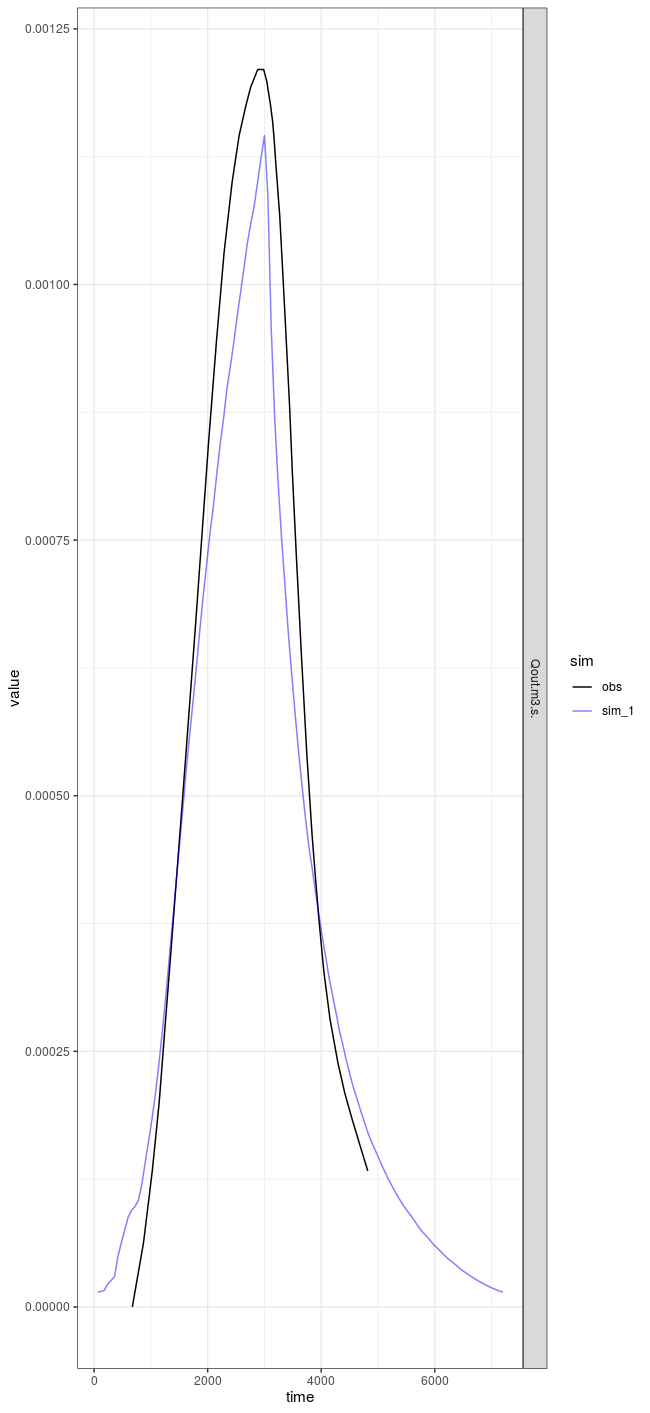
\includegraphics{Borden_v1_files/figure-latex/Comparison-1.png}

Goodness of fit:

\begin{longtable}[]{@{}llr@{}}
\toprule
sim & gof & Qout.m3.s.\tabularnewline
\midrule
\endhead
obs & MAE & 0.00\tabularnewline
obs & RMSE & 0.00\tabularnewline
obs & KGE & 1.00\tabularnewline
sim\_1 & MAE & 0.00\tabularnewline
sim\_1 & RMSE & 0.00\tabularnewline
sim\_1 & KGE & 0.74\tabularnewline
\bottomrule
\end{longtable}

\hypertarget{references}{%
\subsubsection*{References}\label{references}}
\addcontentsline{toc}{subsubsection}{References}

\hypertarget{refs}{}
\begin{cslreferences}
\leavevmode\hypertarget{ref-Abdul1989}{}%
Abdul, A. S., and R. W. Gillham. 1989. ``Field Studies of the Effects of
the Capillary Fringe on Streamflow Generation.'' \emph{Journal of
Hydrology} 112 (1): 1--18.
\url{https://doi.org/https://doi.org/10.1016/0022-1694(89)90177-7}.

\leavevmode\hypertarget{ref-Kollet2017}{}%
Kollet, Stefan, Mauro Sulis, Reed M. Maxwell, Claudio Paniconi, Mario
Putti, Giacomo Bertoldi, Ethan T. Coon, et al. 2017. ``The Integrated
Hydrologic Model Intercomparison Project, Ih-Mip2: A Second Set of
Benchmark Results to Diagnose Integrated Hydrology and Feedbacks.''
\emph{Water Resources Research} 53 (1): 867--90.
\url{https://doi.org/10.1002/2016WR019191}.

\leavevmode\hypertarget{ref-Vanderkwaak2000}{}%
Vanderkwaak, J. E., and E. A. Sudicky. 2000. ``Application of a
physically-based numerical model of surface and subsurface water flow
and solute transport.'' \emph{IAHS-AISH Publication}, no. 265: 515--23.
\end{cslreferences}

\end{document}
